%%%%%%%%%%%%%%%%%%%%%%%%%%%%%%%%%%%%%%%%% 
% Loli Pinel del Valle
% Junio 2015
%%%%%%%%%%%%%%%%%%%%%%%%%%%%%%%%%%%%%%%%%

%----------------------------------------------------------------------------------------
%	MAIN
%----------------------------------------------------------------------------------------

\documentclass[12pt,a4paper,twoside]{book}

\linespread{1.3} %Interlineado
\setlength{\parindent}{1.5cm}  % Longitud de la sangria

%\usepackage[bottom=2.5cm]{geometry} % Required to change the page size to A4
%\geometry{a4paper} % Set the page size to be A4 as opposed to the default US Letter
\usepackage[left=2.5cm,top=2.5cm,right=2cm,bottom=2.5cm]{geometry}

\usepackage[utf8]{inputenc} 
\usepackage[english]{babel}
%\usepackage[spanish]{babel} 

%\usepackage[colorlinks=false,linkcolor=black]{hyperref}
\usepackage[pdftex]{hyperref}

\usepackage{amsmath}
\usepackage{graphicx} % Required for including pictures
\usepackage[small]{caption}  % Letra caption mas pequeña
\usepackage{subfigure}

\usepackage{color} 
\usepackage{float} % Allows putting an [H] in \begin{figure} to specify the exact location of the figure
%\usepackage{wrapfig} % Allows in-line images such as the example fish picture
%\graphicspath{{Pictures/}} % Specifies the directory where pictures are stored


\usepackage{listings} %Para poner código
\usepackage{fancyhdr} % Cabeceras

\pagestyle{fancy}
%%Encabezados
\cfoot{}
\fancyhead[LO]{\nouppercase{\rightmark}}
\fancyhead[RO]{\thepage}
\fancyhead[LE]{\thepage}
\fancyhead[RE]{\nouppercase{\leftmark}}

\renewcommand{\headrulewidth}{0.4pt}

\begin{document}
%%%%%%%%%%%%%%%%%%%%%%%%%%%%%%%%%%%%%%%%%
% Loli Pinel del Valle
% Junio 2015
% Note:
% The \lipsum[#] commands throughout this template generate dummy text
% to fill the template out. These commands should all be removed when
% writing essay content.
%
%%%%%%%%%%%%%%%%%%%%%%%%%%%%%%%%%%%%%%%%%


%----------------------------------------------------------------------------------------
%	TITLE PAGE
%----------------------------------------------------------------------------------------

\begin{titlepage}

\newcommand{\HRule}{\rule{\linewidth}{0.5mm}} % Defines a new command for the horizontal lines, change thickness here

\center % Center everything on the page

\textsc{\LARGE Master Thesis}\\[1.5cm] % Name of your university/college
 
\textsc{\Large Máster en Robótica y Automatización}\\[0.5cm] % Major heading such as course name
\textsc{\large Universidad Carlos III de Madrid}\\[0.5cm]% Minor heading such as course title
\textsc{\large Escuela Politécnica Superior}
\\[2cm]
\HRule \\[0.8cm]
{ \huge \bfseries 
Balance control of humanoid robot TEO using Force/Torque sensors}\\[0.4cm] % Title of your document
\HRule \\[1.5cm]


\large
\emph{Author:}\\
María Dolores Pinel del Valle
\\
\emph{Director:}\\
Santiago Martínez de la Casa Díaz
\vspace{2cm}

{\large Leganés,\\
June 2015}\\[2cm] % Date, change the \today to a set date if you want to be precise

%\includegraphics{Logo}\\[1cm] % Include a department/university logo - this will require the graphicx package

\vfill % Fill the rest of the page with whitespace

\end{titlepage}



%\renewcommand{\tablename}{Tabla}
%\renewcommand{\contentsname}{Índice General}
%\renewcommand{\listfigurename}{Índice de Figuras}
%\renewcommand{\listtablename}{Índice de Tablas}
\renewcommand{\thepage}{\roman{page}}
%\renewcommand{\chaptername}{Capítulo}
%\renewcommand{\bibname}{Referencias}

\setcounter{page}{0}
\tableofcontents
\addcontentsline{toc}{chapter}{\contentsname}


\listoffigures
\addcontentsline{toc}{chapter}{\listfigurename}

\addcontentsline{toc}{chapter}{\listtablename}
\listoftables

\newpage
\setlength{\parindent}{1cm} %Sangria
\renewcommand{\thepage}{\arabic{page}}
\setcounter{page}{0}

\chapter{Introduction}
Industry was one of the first fields of application of robotics, where the environment is mainly static, the tasks to be performed are repetitive and automated, and the human interaction is quite low. For that reason, the idea of designing robots able to work in dynamic environments, with a high variety of tasks and interacting with humans and their environment, was fullfilled thanks to the evolution of new techniques related to robotics. Humanoid robots, physically similar to the human being, meet all that needs. Mainly, the possibility of moving, solves the problem of industrial robots that can only work in fixed areas. Moreover, the provision of artificial intelligence, allows the robot to interact with the surrounding environment in a more natural way, as the human being. \\

%Uno de los primeros campos de aplicación de la robótica fue la industria, donde el entorno del robot es prácticamente estático, las tareas que realiza son repetitivas y automatizadas, y la interacción con el ser humano es relativamente baja. Por ello surgió la necesidad de diseñar robots capaces de trabajar en entornos cambiantes, que sean capaces de realizar tareas de muy diversa índole y que la interactuación con el entorno y el ser humano sea plena. Los robots humanoides, con un aspecto físico similar al del ser humnano, resuelven todas estas últimas necesidades. La posibilidad de desplazarse, a diferencia de los robots industriales, soluciona la problemática de trabajar en un espacio de trabajo fijo. Además, la dotación de inteligencia artificial, permite al robot interactuar con el entorno que lo rodea de una forma mucho más natural para el ser humano.\\

Nevertheless, the posibility of moving, brings 
Sin embargo, la posibilidad de desplazarse trae consigo una gran problemática, la estabilidad. El hecho de que el robot se mantenga erguido y camine, es una tarea complicada desde el punto de vista del control. Sin embargo, para el ser humano, el caminar es una tarea que realiza casi inconsicientemente, por lo que no es consciente de su complejidad. En todo momento, se debe asegurar que el robot se mantenga lo más erguido posible para no caer mientras simultáneamente está realizando una serie de movimientos predefinidos para caminar. Asímismo, ante una situación de desequilibrio, un ser humano, involuntariamente, intenta estabilizarse moviendo el resto de extremidades, lo que es un complicado comportamiento para implementar en un robot.\\

Los primeros trabajos en cuanto a robots bípedos fueron llevados a cabo sobre 1970 por los autores Kato \cite{Kaj} y Vukobratović. El primer robot antropomórfico, WABOT-1, fue exhibido por Kato en 1973 en la Universidad de Waseda (Japón). Usando un esquema de control bastante sencillo, el robot esra capaz de realizar unos pocos pasos lentos, manteniéndose estable en todo momento. Éste logro, fue el primero que desencadenó la investigación acerca de robots humanoides y de su locomoción.\\

Paralelamente, Vukobratović y su equipo investigaban en estabilidad para sistemas bípedos en Yugoslavia, basándose en un nuevo criterio de estabilidad, presentado en 1972, como \textit{Zero-Moment Point (ZMP)}. Teniendo en consideración los efectos dinámicos que se producen durante la caminata, desde entonces hasta la actualidad, el criterio de estabilidad del ZMP ha sido el más utilizado en cuanto a robótica humanoide o bípeda se refiere.\\

El auge de la robótica humanoide comenzó con el desarrollo del robot P2 por la empresa Honda en 1996 \cite{Kaj} . El proyecto comenzó en secreto el proyecto diez años antes, tras el lanzamiento del robot WABOT-2 tocando el piano. P2, de 180 centímetros de altura y 210kg de peso, fue el primer humanoide que podía caminar de forma suficientemente estable y cargar con el procesador y la batería a la espalda. Tras éste, los robots P3 y ASIMO fueron sus versiones avanzadas, reduciendo la estatura y el peso del robot.

\section{Motivacion y objetivos.}
Este Trabajo Fin de Máster tiene como principal objetivo realizar el control de estabilidad del robot humanoide TEO (\textit{Task Environment Operator}) utilizando sensores de Fuerza-Par y tratar los problemas y consideraciones que deben ser tenidas en cuenta cuando se diseña el sistema de control de un robot humanoide.

Los objetivos propuestos son:
\begin{itemize}
\item Puesta en marcha y adquisición de datos en tiempo real de los sensores de Fuerza-Par acoplados a los tobillos del robot, que serán la principal fuente de realimentación del lazo de control.
\item Cálculo de los parámetros de estabilidad de interés, entre ellos el ZMP \textit{Zero-Moment Point}, y evaluar en funcion de éstos la estabilidad o no estabilidad del robot.
\item Diseño de un sistema de control realimentado que permita rectificar los parámetros de estabilidad mencionados anteriormente, y por tanto, la postura del robot para lograr una mayor estabilidad. 
\end{itemize}




\graphicspath{{03_estado_tecnica/Imagenes/}}
\chapter{Literature review}
The performance of the artificial bipedal locomotion is a very complex problem and human beings have the ideal bipedal locomotion. Therefore the best way to produce such a type of motion for a walking machine is to copy human motion.

Human walking is an automated motion, carried out spontaneously. This locomotion process is a repetitive execution until some perturbations are detected. In humans, the muscular system modifies forces acting during the walking in order to maintain equilibrium. The study of the human wakling and the muscles involved in, brings very complex relationships and it requires some simplifications in anthropomorphic legged mechanisms in order to reduce complexity form the mechanical and control points of view.

The analysis of the human walking is fairly recent. McGeer [McGeer 90] built a passive walker around 1990 and showed that his two-legged walker could reproduce stable gait without any controls. However, the most progress was revealed in the active bipedal locomotion [Hirai 98], [Kaneko 2002], [Park 2005]. This type of the locomotion is developed and implemented as artificial human-like bipedal motion based on the previous planning of each step and the real-time automatic control of its execution. 

The basic characteristic of bipedal locomotion is the permanent change of the situation when the mechanism is supported by one foot (single support phase) and when both feet are in contact with the ground (the double support phase). The second situation is statically stable and there are no additional moments affecting the robot. The first situation is statically unstable because when one foot is on the ground, the other is transferred from the back to the front position producing lateral accelerations affecting the mechanism. Thus, the locomotion mechanism changes its structure during a single walking cycle from an open to a closed kinematics chain. Each of these two cases present different dynamical situations and should be taken into account in artificial gait synthesis and control.

As locomotion is a complex task, generally the study of the human body is based in three basic planes: sagital, transversal and frontal (Figure \ref{fig:axes}). It is important to mention that the most important motions related to locomotion occur in the sagital plane because it coincides with the main walking direction. However, the combination of joints of sagital and frontal planes, give the stabilization of the locomotion cycle.

\begin{figure}[!h]
\centering
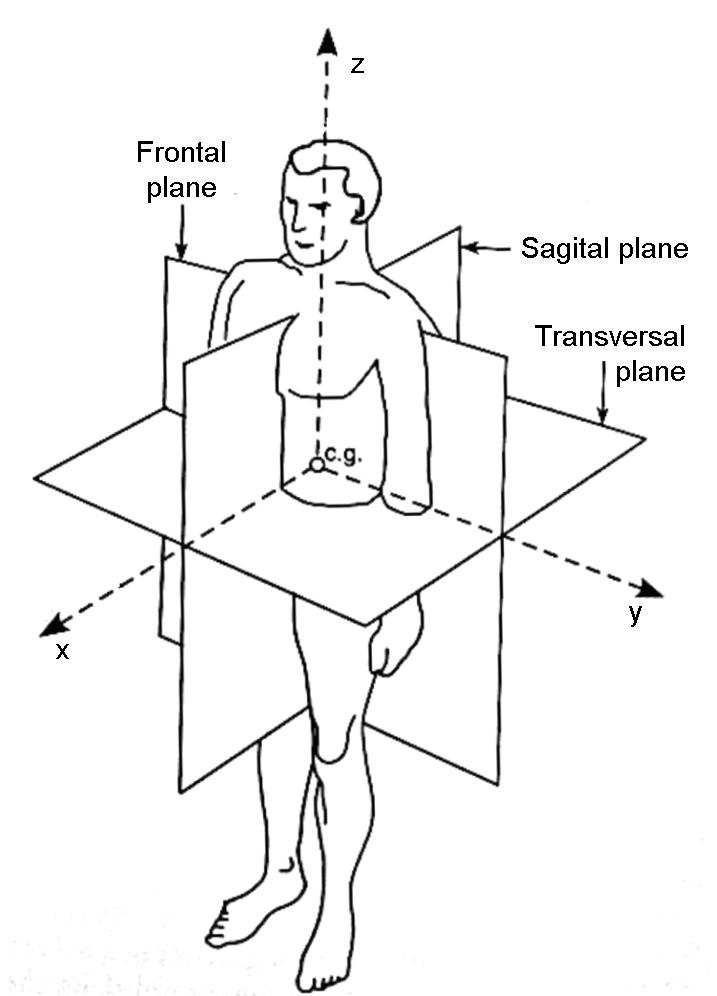
\includegraphics[scale=0.45]{axes.png}
\caption{Axes division of human body.}
\label{fig:axes}
\end{figure}

\section{Bipedal locomotion}
Robot walking, as humans, is performed in a three phase cycle (Fig. \ref{fig:caminata}). The cycle is divided in two, left and right steps. At the begining, the humanoid is in a stable position with both feet on the ground (Fig. \ref{fig:caminata} (a)) and all the body weight is transferred form one foot to the other. Then the step generation starts when the right foot leaves the ground in the swinging phase (Figura \ref{fig:caminata} (b), (c) y (d)). After the right foot touches the ground, the next (right) step with the same basic phases is started, and the whole cycle ends. The single-support phase is the complex one in terms of balance, because all the weight remains in only one support foot.

Swinging phase has also three sub-phases: acceleration, swinging and deceleration (Fig. \ref{fig:caminata} (b), (c) y (d), respectively). The acceleration phase takes its name due to the acceleration of the lifting leg that stops being supported in the ground and gives the impulse to the step. Once the support leg is overtaken, the lifting leg starts the swinging pahse in order to reach the ground with the consequent deceleration.

\begin{figure}[!hbt]
\centering
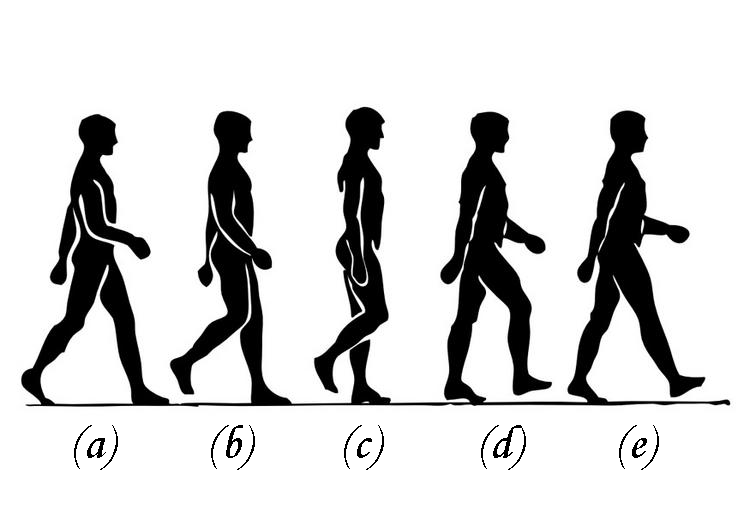
\includegraphics[scale=0.3]{Caminata}
\caption{Phases of biped walking.}
\label{fig:caminata}
\end{figure}

As in the case of the leg, the same occurs with the foot, what adds complexity to control the walking cycle. During a gait, a human foot has four different phases as one can see in Fig. \ref{fig:caminata_pie}. In (a) it is shown how the body weight is supported when the heel is touching the ground. In (b), the foot remains totally plane. In (c), the heel lifts and the weight goes to the front part of the foot. Finally, in (d) the foot is not in contact with the ground and it starts to swing.


\begin{figure}[!hbt]
\centering
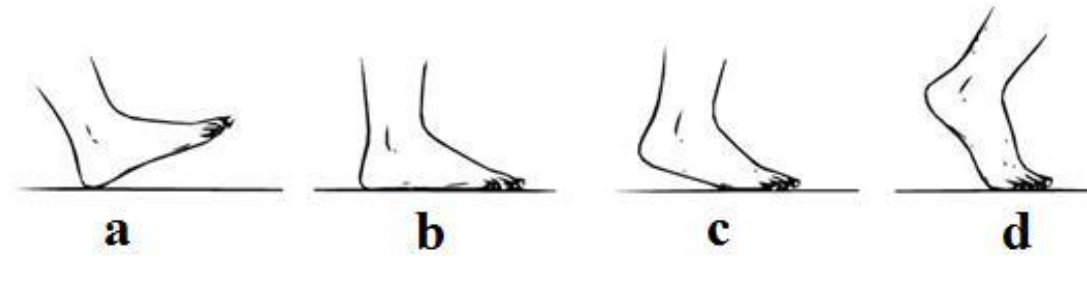
\includegraphics[scale=0.3]{caminata_pie.png}
\caption{Phases of foot support during a walk.}
\label{fig:caminata_pie}
\end{figure}

Almost all humanoid robots do not have articulated feet, due to the high complexity. Mostly they use plane and rigid feet and the control is done in the ankle joint. Some of them, as the robot HRP-4 \cite{Kan}, have a joint called "active toe joint" which allows the movement of the toes. The reason of this improvement is related to reach a more natural and fluent walking, as the human walk.

However, in order to perform a stable walk, is not only necessary the lower body movement. The upper body is also involved in recovery movements. In an example, if a person stumbles. Unwittingly, he or she would move the opposite arm of the unbalanced leg, or even more, moving the torso in order to not to fall down. In the case of a biped robot, the same strategy is followed, what means an high increase of the complexity of the control of the robot stability.

\section{Biped balance/equilibrium}
One of the most important and complex tasks for humanoid locomotion is to avoid overturning during the walking or even to reach an upright position of its body. To prevent that, a necessary and suficient condicion is to ensure that there exists a contact area between the foot and the ground and not a line or a point \cite{Vuk2007}. Given a rectangular-shaped foot, the support area of the robot will be the polygon. In the case that only on foot is touching the ground (single-support), the support area is the contact region between the sole and the ground, i.e., the footprint (Fig. 2.3(a)). On the contrary, when both feet are touching the ground (double-support), the support area will be determined by the footprints and the common tangents between them (Fig. 2.3(b)). It means that in the double-support phase of the walk, the stability area is bigger than in the single-support phase, so the complex of balance control is lower.

\begin{figure}[!hbt]
\centering
\subfigure[Single-support]{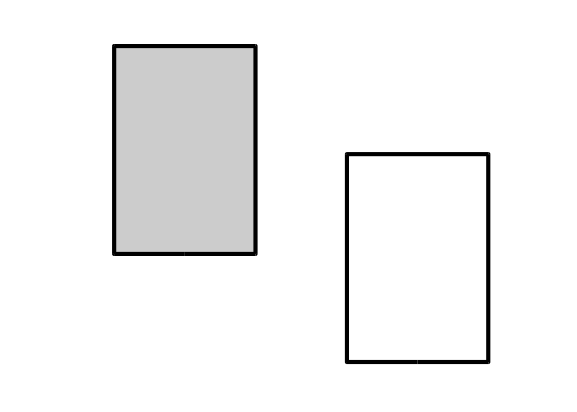
\includegraphics[scale=0.3]{apoyo_simple.png}}
\hspace{10mm}
\subfigure[Double-support]{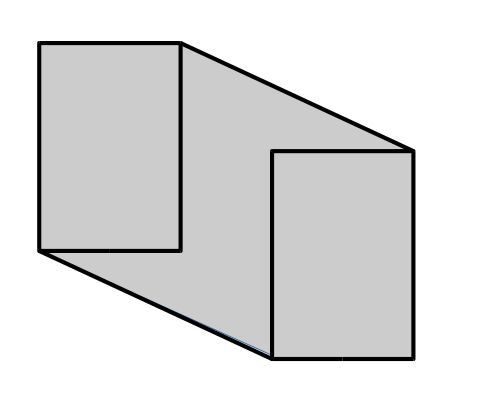
\includegraphics[scale=0.3]{apoyo_doble.png}}
\caption{Support areas depending on the support type.}
\label{fig:apoyo}
\end{figure}

In \cite{Vuk2007}, Vukobratović makes a distinction between the term ``balance" used in the sense of maintaining an upright posture, and ``equilibrium", taking into account the D'Alembert's principle. The D'Alembert's principle states that the resultant of the external forces and the kinetic reaction acting on a body equals zero (condition of kinetic equilibrium). When the humanoid is falling since it is rotating about one foot edge, the D’Alembert’s principle still holds for a point on the foot edge where the pressure force acts. Anyway, this case cannot be contemplated as balanced in the sense of the definition previously provided. This point is called as \textit{Center of Pressure (CoP)} and it is known as the point, in a single-support phase, where the pressure forces (normal to the sole) are equivalent to a single resultant force exerted at the point where the resultant moment is zero.

\section{Zero Moment Point (ZMP)}
From the concept of the CoP, appears a new term known as \textit{Zero-Moment Point (ZMP)}. When a human or a humanoid robot executes a gait during a walk, the ZMP is a point inside the support area where, always, the resulting dynamic reaction of the biped system is acting. In a more specific definition, the ZMP is a point inside the support area where the resultant of all forces and torques acting on the full body, is equal to zero.

Vukobratović \cite{Vuk2007} explains the difference between the CoP and ZMP: CoP and ZMP coincide only when both are inside the support area. When the ZMP goes to the edge of the support area, the humanoid body looses balance and it will fall down. In that case, the ZMP has no sense existing even the CoP.

Goswami \cite{Gos} presented that, mathematically was possible that the point could be outside of the support area and continue satisfying the equilibrium conditions. This point, called \textit{Foot Rotation Indicator (FRI)}, is defined as the point on the contact area between the ground and the foot, inside or outside the suppor area, where the resultant moment of the forces and torques applied on the foot are normal to the surface. Forces and torques applied mean the forces and torques at the ankle joint, and also other external forces, the foot wheight and reaction forces between the foot and the ground. 

However, Vukobratović, on the contrary, stills that the ZMP can only exist inside the support area of the robot. When the ZMP comes close to the edge, any force or moment applied to the system, will produce a rotation about the foot edge and the robot will fall down. In this case, the reaction force of the ground will be at the foot edge and, therefore, it can not be considered as ZMP because there is no stability ensured. That is why the author suggests to denote the point as \textit{Fictitious ZMP} o \textit{FZMP}, if it is outside the support area. 
 
When the robot walking is enough slow to consider almost static, appears the term \textit{pseudo-ZMP}, which is the proyection over the ground of the \textit{Center of Gravity (CoG)} of the system. In such case, lateral accerlerations are so small and can be omitted and the \textit{pseudo-ZMP} = ZMP. Although the \textit{pseudo-ZMP} do not give precise information about the balance of the mecanism, it can be used in order to make a first aproximation in control and design of a humanoid robot.



\subsection{Equations of ZMP}
Let us consider the locomotion mechanism in the single-support phase, with the whole foot being on the ground (Fig. \ref{fig:pie}). To facilitate the analysis we can neglect the part of the mechanism above the ankle of the support foot (point A) and replace its influence by the force $F_A$ and moment $M_A$, whereby the weight of the foot itself acts at its gravity center (point G). The foot also experiences the ground reaction at point P, whose action keeps the whole mechanism in equilibrium.

\begin{figure}[!hbt]
\centering
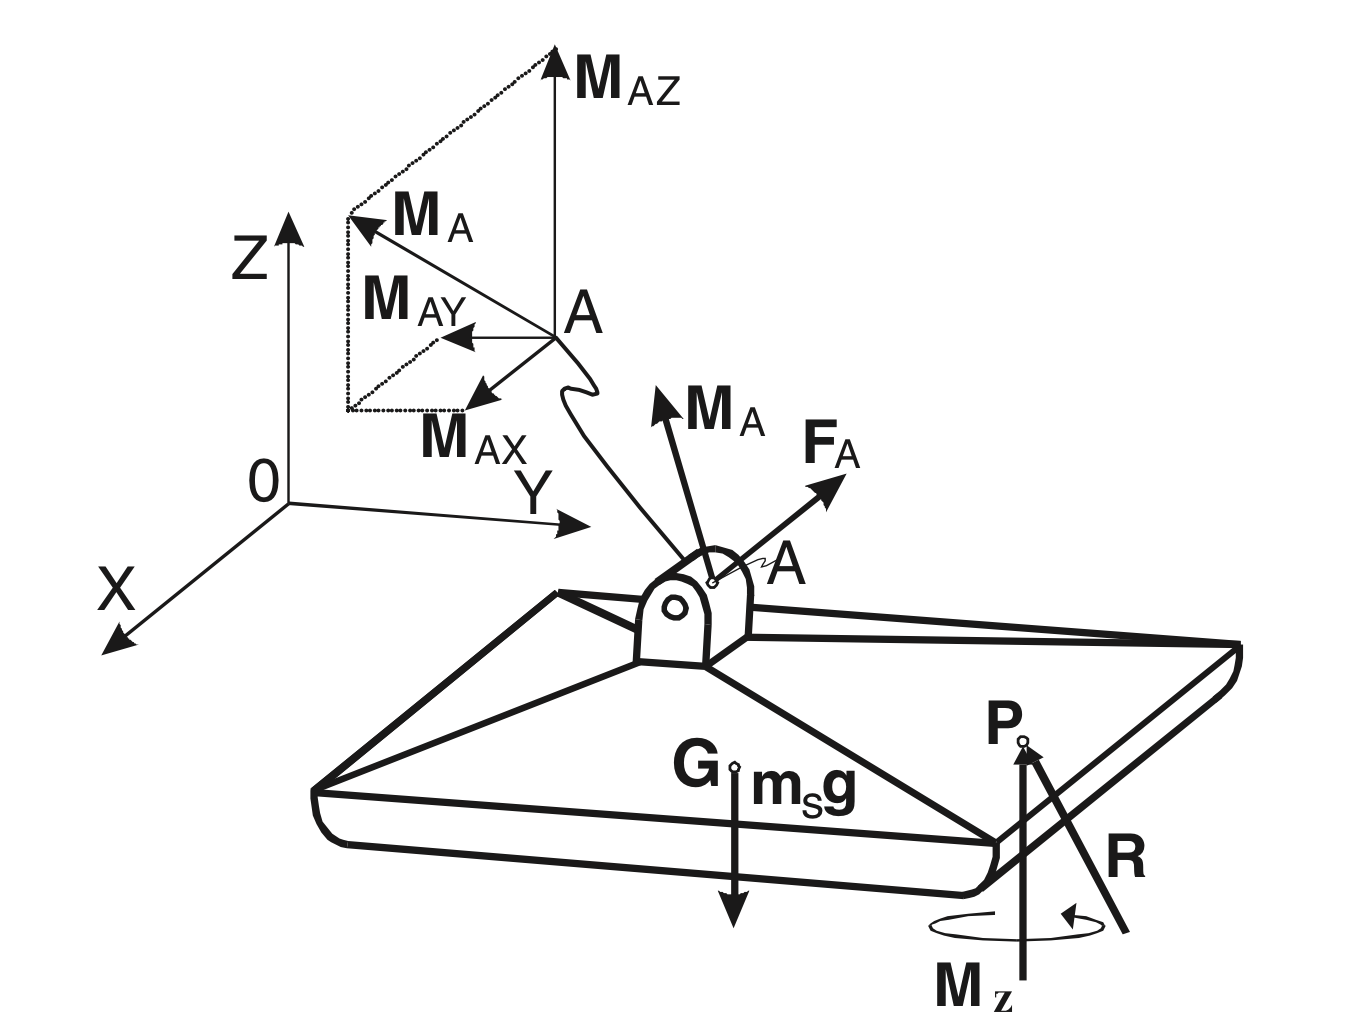
\includegraphics[scale=0.4]{pie.png}
\caption{Forces acting on the foot of the bipedal mecanism \protect\cite{Vuk2004} }
\label{fig:pie}
\end{figure}

In general, the total ground reaction consists of three components of the force $R (R_x, R_y, R_z)$ and moment $M (M_x, M_y, M_z)$ exerted at the foot-ground contact point. During the support phase, it is assumed there is no shifting in the contact point, which means that horizontal reaction force $R_x$ and $R_y$ balances the horizontal component of the force $F_A$, whereas the vertical reaction moment $M_z$ represents the moment of friction reaction forces that balances the vertical component of the moment $M_A$ and the moment induced by the force $F_A$.

However, due to a unidirectional nature of the connection between the foot and the ground (it is obvious that the ground reaction force induced by foot action is always oriented upwards) horizontal components of all active moments ($M_A$) can be compensated for only by changing position of the reaction force $R$ within the support polygon. This is illustrated in Fig. \ref{fig:pieYOZ} where a planar case in $y-z$ plane is represented.

\begin{figure}[!hbt]
\centering
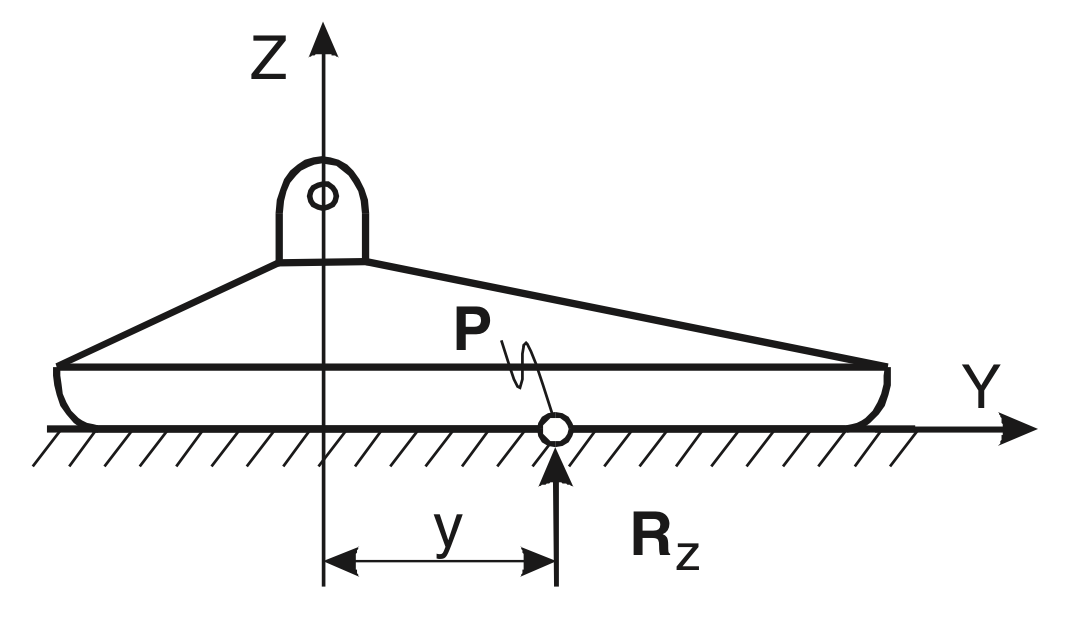
\includegraphics[scale=0.4]{pieYOZ.png}
\caption{Compensación $M_{Ax}$ \protect\cite{Vuk2004} }
\label{fig:pieYOZ}
\end{figure} 

The moment $M_{Ax}$ is balanced by shifting the acting point of the force $R_z$, whose intensity is determined from the equation of balance of all the forces acting on the foot, by the corresponding distance y. It is necessary to emphasize that all the time the reaction force is within the area covered by the foot, the increase in the ankle moment will be compensated for by changing the position of this force $R_z$, and no horizontal components of the moments $M_x$ and $M_z$ will exist. This is the reason why in Fig. \ref{fig:pie} at point $P$ only the $M_z$ component exists.

However, if the real support polygon is not large enough to encompass the appropriate position of the force $R$ to balance the action of external moments, the force $R$ will act at the foot edge and the uncompensated part of the horizontal component of the reaction moment will cause the mechanism’s rotation about the foot edge, which can result in the mechanism’s overturning. Therefore, it can said that the necessary and sufficient condition for the locomotion mechanism to be in dynamic equilibrium is that for the point $P$ on the sole where the ground reaction force is acting,

\begin{equation}
M_x = 0;
M_y = 0.
\end{equation}

That is why the \textit{Zero-Moment Point} is called the contact point with the ground ($P$) where there no exist shifting, i.e., moments $M_x$ y $M_y$ are zero.

From Fig. \ref{fig:pie} static equilibrium equations for the supporting foot are obtained:
\begin{equation}
\sum \overrightarrow{F} = 0 \Rightarrow \overrightarrow{R} + \overrightarrow{F_A} + m_s g = 0
\label{eq:fuerzas}
\end{equation}
\begin{equation}
\sum \overrightarrow{M_O} = 0 \Rightarrow \overrightarrow{OP} \times \overrightarrow{R} + \overrightarrow{OG} \times m_sg + M_A + M_z + \overrightarrow{OA} \times F_A = 0,
\label{eq:momentos}
\end{equation}

where $\overrightarrow{OP}$, $\overrightarrow{OG}$ and $\overrightarrow{OA}$ are radius vectors from the origin of the coordinate system $O_{xyz}$ to the ground reaction force acting point ($P$), foot mass center ($G$), and ankle joint ($A$), respectively, while the foot mass is $m_s$. If we place the origin of the coordinate system at the point $P$ and project Eq. \ref{eq:momentos} onto the z-axis, then the vertical component of the ground reaction momentc (actually, it is the ground friction moment) will be

\begin{equation}
M_z = M_{fr} = -M_A^Z + (\overrightarrow{OA} \times F_A)^Z
\end{equation}

In a general case, this moment is different from zero and can be reduced to zero only by the appropriate dynamics of the overall mechanism. However, the projection of Eq. \ref{eq:momentos} onto the horizontal plane gives:
\begin{equation}
(\overrightarrow{OP} \times \overrightarrow{R})^H + \overrightarrow{OG} \times m_sg + (M_A)^H + (\overrightarrow{OA} \times F_A)^H = 0,
\label{eq:momentos}
\end{equation}
This equation is a basis for computing the position of the ground reaction force acting point ($P$) which gives the ZMP position.


\subsection{Relation between COG and ZMP}
When a humanoid robot is in the single-support phase during a walking cycle, its dynamics can be represented by a single inverted pendulum where the supporting foot is the point where all body mass is concentrated (COG) and a mass less telescopic leg \cite{Kaj2001}. The pendulum can increase or decrease its length, thus simulating the functioning of the ankle joint.

Now, let us consider that the inverted pendulum instead of only one contact point considered above, has a contact polygon as the surface in contact with the ground (Fig. \ref{fig:3DLIPM}).

\begin{figure}[!hbt]
\centering
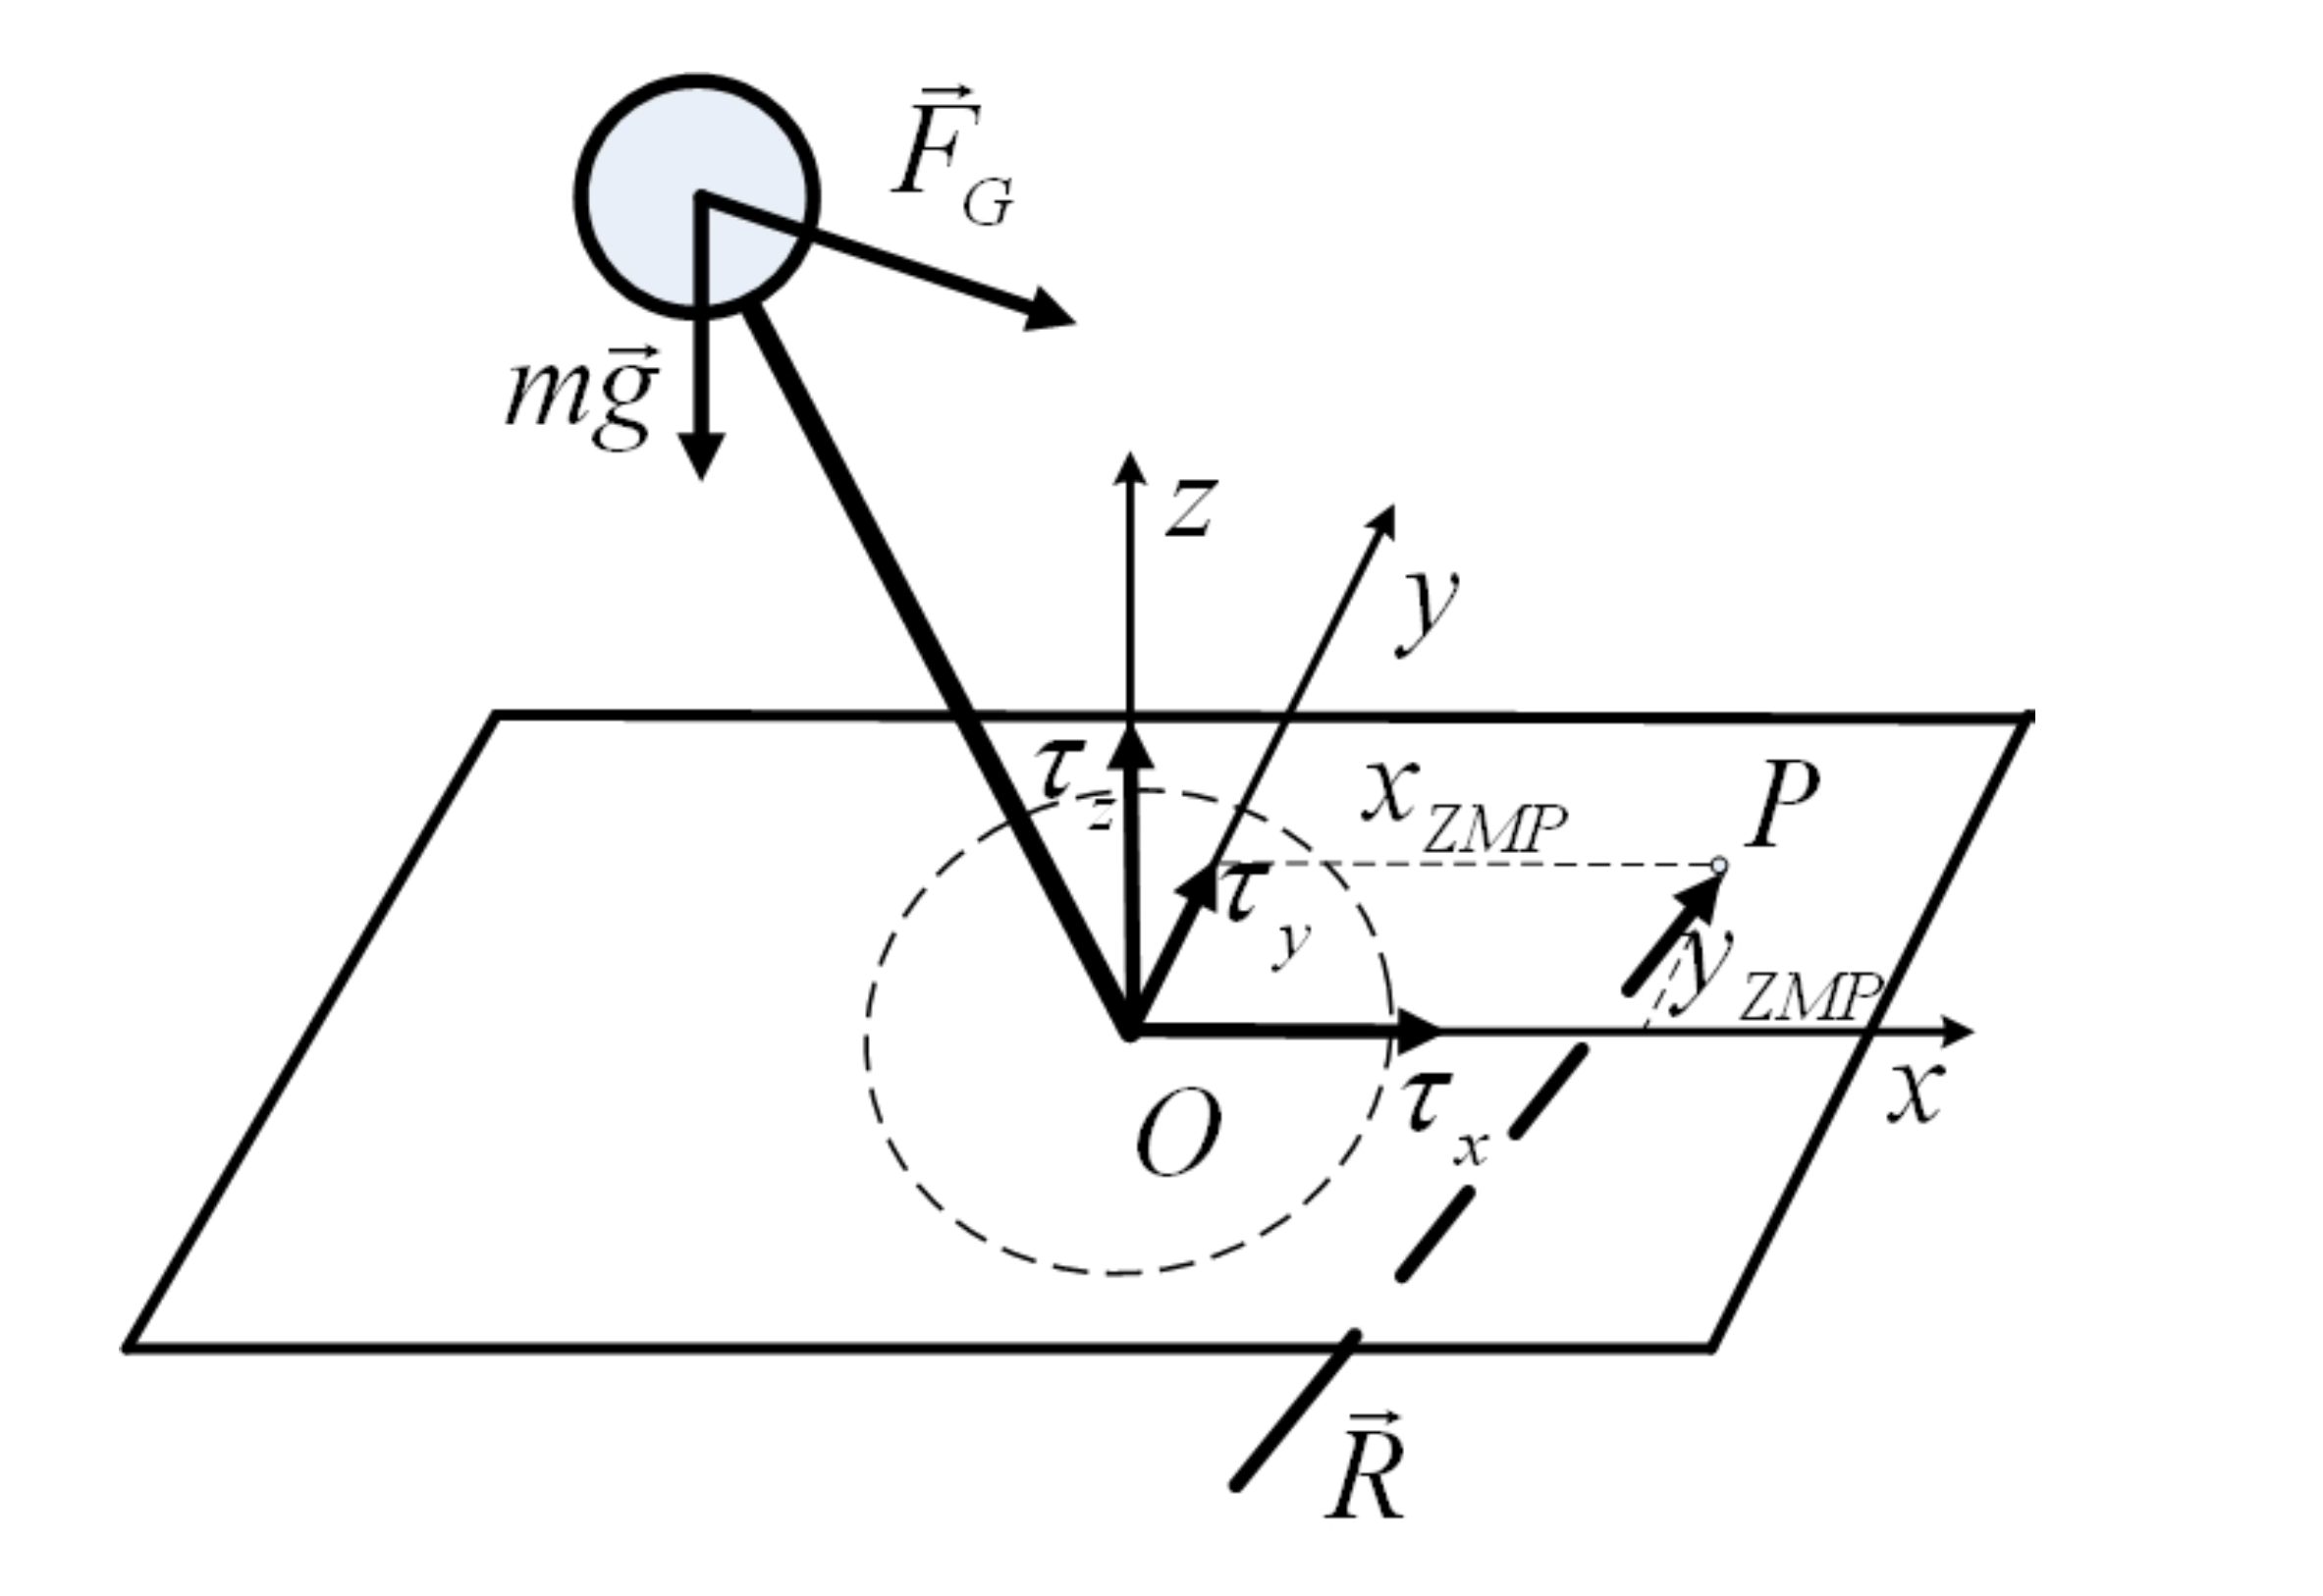
\includegraphics[scale=0.2]{3DLIPM.png}
\caption{3D Linear Inverted Pendulum with a contact polygon. \textcolor{red}{CITA}}
\label{fig:3DLIPM}
\end{figure}

Inertial $\overrightarrow{F_G}$ and gravity $m\overrightarrow{g}$ froces act on the point mass located in the COG of the humanoid robot. The contact of the pendulum with the ground produces a reaction force $\overrightarrow{R}$ and reaction moment $\overrightarrow{M_P}$ at point $P$ For any other point of the support polygon (taking point 0 as origin), the moment $M_0=[\tau_x, \tau_y, \tau_z]^T$ produced by the ground reaction force $\overrightarrow{R}$ is represented: 
\begin{equation}
M_0 = M_P + \overrightarrow{0P} \times \overrightarrow{R}
\label{eq:M0}
\end{equation}

If it is considered point P to be the ZMP of the system, then from the interpretation of the ZMP presented above $M_P = 0$. In this case we can denote vector $\overrightarrow{OP} = [x_{ZMP}, y_{ZMP}, z_{ZMP}]^T$ and eq. \ref{eq:M0} gives the following equation:
\begin{equation}
\begin{pmatrix}
\tau_x \\
\tau_y \\
\tau_z 
\end{pmatrix} 
=
\begin{pmatrix}
x_{ZMP} \\
y_{ZMP} \\
z_{ZMP}
\end{pmatrix}
\times \overrightarrow{R}
\label{eq:1}
\end{equation}

From the other side, applying Newton’s law of mechanics to system in Fig. \ref{fig:3DLIPM}:
\begin{equation}
m \overrightarrow{a_G} = \overrightarrow{R} - m\overrightarrow{g}
\label{eq:newton}
\end{equation}

where $\overrightarrow{a_G} = [\ddot{x}, \ddot{y}, \ddot{z}]^T$ is the acceleration of the COG. From \ref{eq:newton} it is obtained:
\begin{equation}
\overrightarrow{R} = m 
\begin{pmatrix}
\ddot{x} \\
\ddot{y} \\
\ddot{z} + g
\end{pmatrix}
\label{eq:2}
\end{equation}

Substituting equation \ref{eq:2} into the equation of balance of moments \ref{eq:1} it is obtained:
\begin{equation}
\begin{pmatrix}
\tau_x \\
\tau_y \\
\tau_z 
\end{pmatrix} 
= m
\begin{pmatrix}
x_{ZMP} \\
y_{ZMP} \\
z_{ZMP}
\end{pmatrix}
\times
\begin{pmatrix}
\ddot{x} \\
\ddot{y} \\
\ddot{z} + g
\end{pmatrix}
\end{equation}

After a cross product and taking into account that $z_{zmp} = 0$, because the ZMP lies into the ground:
\begin{equation}
\begin{pmatrix}
\tau_x \\
\tau_y \\
\tau_z 
\end{pmatrix} 
= m
\begin{pmatrix}
y_{ZMP}(\ddot{z}+g) \\
-x_{ZMP}(\ddot{z}+g) \\
x_{ZMP}\ddot{y}-y_{ZMP}\ddot{x}
\end{pmatrix}
\label{eq:3}
\end{equation}

From \eqref{eq:3}, it can be stated the ZMP position of the system:
\begin{equation}
x_{ZMP} = -\frac{\tau_y}{m(\ddot{z}+g)}
\label{eq:x}
\end{equation}
\begin{equation}
y_{ZMP} = \frac{\tau_x}{m(\ddot{z}+g)}
\label{eq:y}
\end{equation}

If it is supposed that the COG always remains within the horizontal plain intersecting the $z$ axis in the point $z_c$ (one of the constraints of the 3D-LIPM model), then the vertical component of the COG acceleration $\ddot{z}=0$. Then, finally, equations \ref{eq:x} and \ref{eq:y} take the form:
\begin{equation}
x_{ZMP} = -\frac{\tau_y+hF_x}{mg}
\label{eq:xzmp}
\end{equation}
\begin{equation}
y_{ZMP} = \frac{\tau_x+hF_y}{mg}
\label{eq:yzmp}
\end{equation}
where $h$ is the distance between the ground and the measuring point, i.e, the height of the sole. 
These are the \textit{ZMP equations}, without forgetting it was considered before that lateral accelerations of the COG $\ddot{x}=0$ and $\ddot{y}=0$. One can see that moments $\tau_x$ and $\tau_y$ in $x$ and $y$ directions respectively affect the ZMP position of the mecanism and it can loose balance because of their change.

If we take into account these lateral accelerations of the COG, the ZMP can be expressed as a function of the acceleration of the COG as: \textcolor{red}{REFERENCIA?}
\begin{equation}
x_{ZMP}=x-\frac{z_c}{g}\ddot{x}
\end{equation}
\begin{equation}
y_{ZMP}=y-\frac{z_c}{g}\ddot{y}
\end{equation}

These equations can only be applied to compute ZMP in single-support phase. In the case of the double-support phase, it is necessary to calculate the weighted average of the sensor measurements form both feet as recommended in \cite{Kaj2005}. Therefore, the resulting equations for ZMP in double-support phase are:

\begin{equation}
x_{ZMP} = -\frac{F_{y}^{R}\cdot x^{R}+F_{y}^{L}\cdot x^{L}}{F_{z}^{R}+F_{z}^{L}}
\end{equation}
\begin{equation}
y_{ZMP} = \frac{F_{x}^{R}\cdot y^{R}+F_{x}^{L}\cdot y^{L}}{F_{z}^{R}+F_{z}^{L}}
\end{equation}
where the upper index $R$ represents the right foot and $L$ the left one.
\textcolor{red}{Revisar si el numerador es par o fuerza}.

\subsection{ZMP areas.}
As mentioned before, ZMP is a point in the sole which depends on the forces and moments applied to the robot. Therefore, depending on the magnitude of that forces, ZMP will change and it becomes a dynamic parameter. As suggested in \cite{Vuk2007}, three regions are defined depending on the position of the ZMP as one can see in Fig. \ref{fig:zonas}.
In the balanced area (safe region), the control action will not actuate. In the nearly critical region, the control action will actuate as a secondary solution. This may be the case of a walking task. As humans do, the robot may use its arms in order to reduce the zero-moment point position closer to the safe region. Finally, in the critical region, the stabilizer will actually disconnect the ongoing task and actuate on the full body. Even if this region is still stable, the balance may be easily lost. 


\begin{figure}[!hbt]
\centering
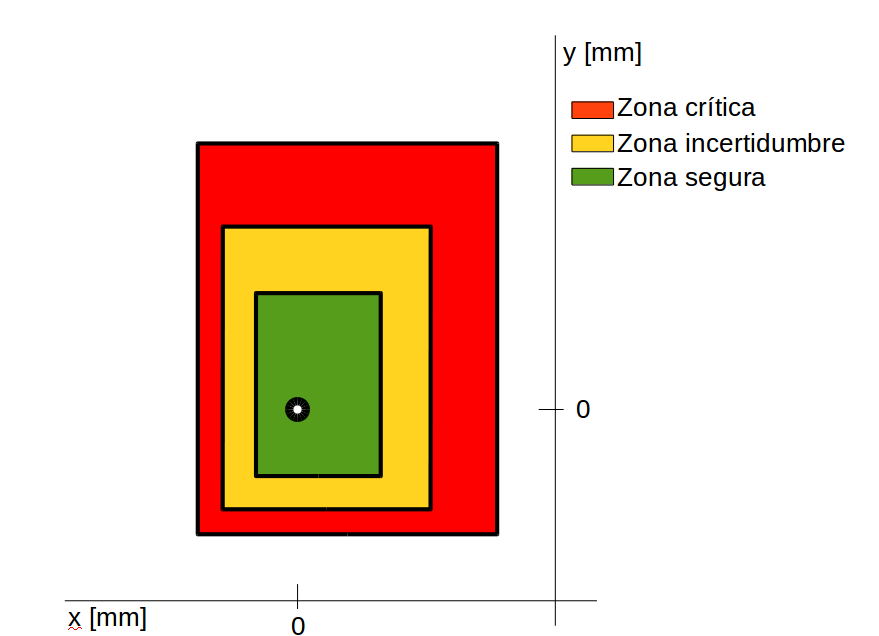
\includegraphics[scale=0.3]{zonas}
\caption{ZMP stability regions in single-support.}
\label{fig:zonas}
\end{figure}



\section{Biped modeling}
Humanoid robots have a very complex dynamics because of their complex mechanical configuration and they require a high computational cost. Figure ??? represents a simplified mechanical configuration of a typical humanoid robot. As one can see, the high number of DOFs due to the precise knowledge of robot dynamics including, mass, location of the centre of mass and moments of inertia of each link, make stable biped locomotion very complex. Thus, different simplified models of the mechanics have been developed. These methods use limited knowledge of the dynamics and the humanoid is usually represented by a planar inverted pendulum with the base representing the ankle joint and, in case of 3D locomotion, the Three-Dimensional Inverted Pendulum Mode (3D-LIPM) \cite{Kaj2001}.

\graphicspath{{04_plataforma/Imagenes/}}

\chapter{Platform description}
\section{Humanoid robot TEO}
Humanoid robot RH-2, also known as TEO (Task Environment Operator), from University Carlos III of Madrid, is and advanced version of humanoid robots RH-0 and RH-1. TEO is 165 cm high overtaking 150 cm of RH-1 and 120 cm of RH-0. It wheights about 60 kg and it can carry about 2 kg of payload. It has 24 DOFs (26 DOFs taking into account head motors), 3 more DOFs than in previous RH versions. In Figure \ref{ref:gdl} one can see the robot DOFs, besides their movements, being 6 DOFs for each leg, 6 DOFs for each arm, 2 DOFs for the torso and 2 DOFs for the head.

\begin{figure}[!hbt]
\centering
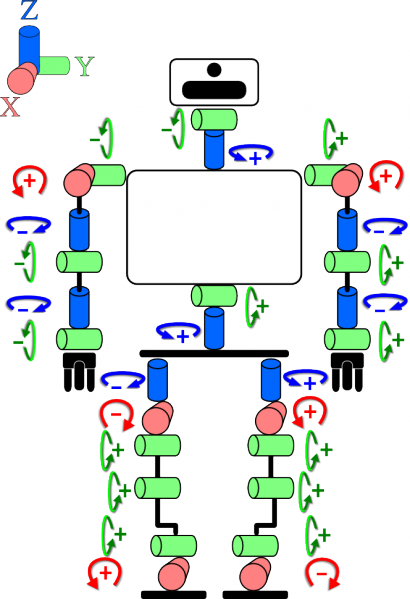
\includegraphics[scale=0.45]{teo_gdl.png}
\caption{Distribución de grados de libertad del robot TEO.}
\label{fig:gdl}
\end{figure}

The robot has 4 microprocessors: locomotion, manipulation, artificial vision tasks and last, the main processor which manages the others. The locomotion processor, that controls the legs and the torso, will be responsible for getting the sensors information and maintain the robot in a balance and upright position, being static or in a walking cycle. The manipulation processor controls the movement of the arms and the head. The processor responsible for the computer vision uses a camera with infrarred sensor ASUS located in the head.

The communication system is based on the CAN-bus protocol. Making a sagittal and transversal division, there are 4 CAN-bus lines: 1 line per each arm and neck, and 1 line per each leg and torso.

For data acquisition, the robot has Force-Torque sensors located at the robot ankles and wrists, used locomotion and manipulation, respectively. These sensors are plugged into real time data acquisition PCI cards. Including F/T sensors is an important difference and advantage respect RH-2 predecessors. They allow to close the control loop and then, to obtain a kind of feedback which is necessary to accomplish tasks successfully.


\section{Force/Torque sensors}
Force-Torque (F-T) sensors are based on strain gauge sensors arranged in such a way that allows to obtain force and moment measures in all axes of the 3D space. 

The sensors used in the platform, are the commercial JR3 F-T sensors described in Table\ref{table:sensores}. Look at the full scales difference between the sensors used in the wrists joints and the ones used in the ankle joints. Ankle sensors must be able to support greater forces and moments including the ones exerted by the own robot.

\begin{table}[!hbt]
\centering
\begin{tabular}{|cl|c|c|c|c|}
\hline
Joint & Model & $F_{x,y}$ & $F_z$ & $M_{x,y,z}$\\
\hline
Wrist & 50M31A & 100N & 200N & 5 Nm\\ 
\hline
Ankle & 85M35A & 250N & 500N & 212Nm\\
\hline
\end{tabular}
\caption{F-T sensor models and characteristics. [JR3 Inc.]}
\label{table:sensores}
\end{table}

According to the manufacturer, the two first digits of the model show the sensor diameter, followed by the serie, and the next two digits, the thickness. As mentioned before, the ankle sensors are bigger and they support greater forces and moments. The sensors used in this Master Thesis are the ones mentioned in Table \ref{table:sensores} for ankle joints.

Serie M sensors include inner electronics in order to filter noise, digital output to use a data acquisition PCI card from the same manufacturer and an analogical output option. The nominal precission of all sensors of serie M is 1\% of full scale, and a 1/4000 full scale resolution.

The sensors used in this work, provide the option of acquiring data in International System Units or Imperial System Units, according to Figure \textcolor{red}{FIGURA}.

\section{Data Acquisition}
The PCI cards used for data acquisition are PCI 1592D from JR3 Inc, which has 4 ports (named as in Figure ???). The sensors are plugged through a 6 or 8 pinout cables (RJ-11 and RJ-45, respectively). In the case of RJ-45, two pinouts are not used. The PCI card uses these cables to receive high speed data and provide power supply to the sensors. About the PCI supply, it is provided by the PCI slot form the computer where it is installed.

In order to access to received data from the sensors, it is necessary to access to card memory, specifying the memory address for each available data. These addresses can be found at [ANEXO. DATOS DEL FABRICANTE].

It is important to take into account that the forces and torques obtained from the sensors and processed by the card, are in the International System Units. Forces are given in Newton [N] and torques are given in tenths of a newton per meter [dN·m].

\subsection{Acquisition program}
The data acquisition of forces and moments form the sensors is done by user programs by means of the data aquisition card. 

The \textit{jr3pci2channelYarp} program (See ANEXOS) reads data from 2 Force/Torque Sensors with a rate of $40 \mu s$.

The sequence of the program is the following: reads data from sensors, scales the data to SI units, clusters the data into a YARP Bottle object and sends it through YARP ports.

\addcontentsline{toc}{chapter}{Bibliography}
\begin{thebibliography}{X}


\bibitem{Gos} Goswami A., “Foot Rotation Indicator (FRI) point: A new gait planning tool to evaluate postural stability of biped robots,” in Proceedings of the IEEE International Conference on Robotics and Automation, (Detroit, Michigan, USA), pp. 47–52, IEEE, 1999.

\bibitem{Kaj_2001} Kajita S., Kanehiro F., Kaneko K., Yokoi K. and Hirukawa H., The 3D Linear Inverted Pendulum Mode: A simple modeling for a biped walking pattern generation. In Proc. IEEE Conf on Intelligent Robots and Systems (IROS 2001), pp. 239-246, Hawaii, 2001. 

\bibitem{Kaj_2005} Kajita S. et al, "Introduction to Humanoid Robotics", Springer Tracts in Advanced Robotics, Springer, 2005.

\bibitem{Kan} Kaneko, K. et al. "Hardware improvement of Cybernetic Human HRP-4C for entertainment use", IEEE International Conference on Intelligent Robots and Systems, (San Francisco, California, USA), pp. 4392-4399, IEEE 2011.

\bibitem{Vuk} Vukobratović, M.; Borovac, B.; and Potkonjak, V. “Towards a unified understanding of basic notions and terms in humanoid robotics,” Robotica, vol. 25, pp. 87–101, 2007. \textcolor{red}{Falta articulo.}

\bibitem{Vuk_2004} Vukobratović, M.; Borovac, B. "Zero-Moment Point: Thirty five years of its life". International Journal of Humanoid Robotics. Vol. 1, No. 1, pp. 157-173, 2004
\end{thebibliography}


\end{document}

